% UzGenABSA: Large Language Models for Aspect-Based Sentiment Analysis
% of Uzbek Service-Sector Reviews
% MSBC-2026 submission, Springer LNCS format
%
\documentclass[runningheads]{llncs}

\usepackage[T1]{fontenc}
\usepackage[utf8]{inputenc}
\usepackage{graphicx}
\usepackage{booktabs}
\usepackage{array}
\usepackage{multirow}
\usepackage{xcolor}
\usepackage{amsmath}
\usepackage{amssymb}
\usepackage{tabularx}
\usepackage{listings}
\usepackage{url}
\usepackage{microtype}
\usepackage{placeins}
\usepackage[hidelinks]{hyperref}
\usepackage{tikz}
\usetikzlibrary{arrows.meta,positioning}

% Relax float placement so tables/figures land near their text
\renewcommand{\topfraction}{0.95}
\renewcommand{\bottomfraction}{0.85}
\renewcommand{\textfraction}{0.05}
\renewcommand{\floatpagefraction}{0.6}
\setcounter{topnumber}{3}
\setcounter{bottomnumber}{2}
\setcounter{totalnumber}{5}

% URL style (per LNCS guidance)
\renewcommand\UrlFont{\color{blue}\rmfamily\itshape}

% Lightweight code-listing style for the JSON / prompt boxes
\lstdefinestyle{absajson}{
  basicstyle=\ttfamily\scriptsize,
  breaklines=true,
  columns=fullflexible,
  keepspaces=true,
  showstringspaces=false,
  frame=single,
  rulecolor=\color{gray!40},
  framerule=0.3pt,
  xleftmargin=4pt,
  xrightmargin=4pt,
  aboveskip=4pt,
  belowskip=4pt
}
\lstset{style=absajson}

\begin{document}

\title{Large Language Models for Aspect-Based Sentiment Analysis of Uzbek Service Sector Reviews}

\titlerunning{LLMs for Aspect-Based Sentiment Analysis of Uzbek Service Reviews}

\author{Mersaid Aripov\inst{1}\orcidID{0000-0001-5207-8852} \and
Sanatbek Matlatipov\inst{1}\orcidID{0000-0002-6895-3436}}

\authorrunning{M. Aripov and S. Matlatipov}

\institute{National University of Uzbekistan, Tashkent, Uzbekistan\\
\email{mirsaid.aripov@nuu.uz, s.matlatipov@nuu.uz}}

\maketitle

\begin{abstract}
Online consumer reviews are a primary form of digitally mediated
social-behavioural data, yet for low-resource languages such as Uzbek the
signal is largely inaccessible due to the absence of fine-grained sentiment
resources. We present \textbf{UzGenABSA}, an end-to-end framework that
fine-tunes open-source LLMs with QLoRA for Aspect-Based Sentiment Analysis
(ABSA) on Uzbek service-sector reviews and turns the strongest model into a
scalable multi-domain annotation engine. Under an identical QLoRA
configuration we compare Qwen-2.5-7B, Llama-3.1-8B and
DeepSeek-R1-Distill-Qwen-7B against their own zero-/few-shot baselines on a
618-sentence test split; fine-tuned Qwen reaches ATE-F1 0.660 with a 100\%
JSON parse rate, while Llama reaches the best aspect--polarity F1 0.581 and
sentiment accuracy 0.886. Strikingly, validation cross-entropy ranking does
not match ABSA task ranking. We then deploy the strongest model over 5{,}038
multi-domain reviews (23 business categories), score 307 of them with a
GPT-4o-mini LLM-as-Judge five-dimensional rubric, and human-verify 50
reviews (94\% gold-agreement, Spearman $\rho{=}0.71$ judge--human). The
resulting silver corpus of 9{,}884 aspects surfaces sector-specific
satisfaction patterns in banking, retail and HoReCa directly interpretable
as social signals. We release the dataset, code and adapters.

\keywords{Aspect-Based Sentiment Analysis \and Large Language Models \and
Uzbek \and Low-resource NLP \and QLoRA \and LLM-as-Judge \and Social-behavioural data.}
\end{abstract}

%====================================================================
\section{Introduction}
\label{sec:intro}

The rapid expansion of digital platforms has transformed online consumer
reviews into a primary source of social-behavioural data. Citizens use these
platforms to evaluate services, articulate satisfaction or dissatisfaction,
and communicate expectations toward businesses and public institutions. In
emerging digital societies, such reviews can support evidence-based service
improvement and offer a window into how trust and quality of experience are
constructed in everyday interactions~\cite{Hua2024,ZohrehMadhoushi2019}.

For low-resource languages, however, this signal is largely inaccessible.
Aspect-Based Sentiment Analysis (ABSA)~\cite{pontiki-etal-2014-semeval}, the
task of jointly identifying \emph{what} is being evaluated (an
\emph{aspect}) and \emph{how} it is evaluated (its \emph{polarity}), is the
natural computational lens for this kind of analysis because it preserves
fine-grained social information that flat positive/negative classification
discards. Yet ABSA research is dominated by English and a handful of
high-resource languages~\cite{Hua2024}, and Uzbek -- a Turkic, agglutinative
language with a dual Latin/Cyrillic literacy and an emerging digital
ecosystem -- remains a striking blind spot. Multilingual encoders such as
mBERT and XLM-R offer only marginal Uzbek
representation~\cite{devlin-etal-2019-bert,blasi-etal-2022-systematic};
domain-adapted Uzbek BERTs exist~\cite{kuriyozov-etal-2024-bertbek,Mamasaidov2023TahrirchiBERT} but are general-purpose and have not been
applied to token-level ABSA. The first dedicated Uzbek ABSA dataset, UzABSA,
was released only recently~\cite{matlatipov2024uzabsa} and covers a single
domain (restaurant reviews).

Two recent technical developments make it timely to bridge this gap.
First, open-weight LLMs at the 7--8B parameter scale (Qwen-2.5~\cite{Qwen2024-kr},
Llama-3.1~\cite{Grattafiori2024-ka}, DeepSeek-R1
distillations~\cite{DeepSeek-AI2026-vt}) show emergent cross-lingual
generalisation, and instruction-tuned ABSA~\cite{scaria-etal-2024-instructabsa,10.1145/3777411} reformulates ABSA as constrained text generation, side-stepping
the need for tag-set engineering. Second, parameter-efficient fine-tuning
through QLoRA~\cite{10.5555/3666122.3666563} reduces a 7B fine-tuning job to
$<6$\,GB of GPU memory, which makes systematic comparison feasible even
under low-resource computational budgets.

We bring these two threads together for Uzbek and frame the result as
\emph{computational social-behavioural research}. Our contributions are the
following.

\begin{enumerate}
\item \textbf{First systematic LLM-based ABSA study for Uzbek.} We fine-tune
and compare three open-source LLMs (Qwen-2.5-7B, Llama-3.1-8B,
DeepSeek-R1-Distill-Qwen-7B) under an identical QLoRA configuration on the
UzABSA SemEval-2014-style corpus, and benchmark them against their own
zero-shot and 3-shot baselines.

\item \textbf{A scalable model-assisted annotation pipeline.} We chain the
best fine-tuned model (Qwen-2.5-7B, 100\% JSON parse rate) with an
LLM-as-Judge quality layer (GPT-4o-mini, five-dimensional
rubric)~\cite{10.5555/3666122.3668142,2506.22316} and a human verification
sample, producing a quality-tiered silver standard at a marginal cost.

\item \textbf{A novel multi-domain silver Uzbek ABSA dataset.} 5{,}038
reviews spanning 23 business categories (banking, retail, HoReCa, telecom,
healthcare, education, e-commerce, transport, $\ldots$) are released with
9{,}884 aspect--sentiment pairs, per-review judge scores, and provenance
metadata.

\item \textbf{Empirical and social-behavioural findings.} (i) Training
cross-entropy ranking does not match ABSA task ranking, which has
implications for model selection in structured extraction. (ii) A
restaurant-trained model generalises to 15 of 23 service domains above an
LLM-judged inclusion threshold, with quality degrading along a measurable
in-domain $\to$ near-domain $\to$ specialised-domain gradient. (iii)
Aspect-level satisfaction patterns are sector-specific and directly
interpretable as actionable evidence for service redesign.
\end{enumerate}


%====================================================================
\section{Related Work}
\label{sec:related}

\paragraph{ABSA: from sequence labelling to instruction tuning.}
ABSA was formalised by the SemEval-2014 Task~4 shared
task~\cite{pontiki-etal-2014-semeval}, which decomposed the problem into
Aspect Term Extraction (ATE), Aspect Category Detection (ACD), Aspect
Sentiment Classification (ASC) and end-to-end joint extraction. Subsequent
work explored sequence-to-sequence
formulations~\cite{ma-etal-2019-exploring},
graph-convolution models~\cite{10.1145/3721844}, few-shot category
detection~\cite{hu-etal-2021-multi-label} and BERT-based joint
models~\cite{electronics12030515}. Recent surveys~\cite{Hua2024,ZohrehMadhoushi2019} report that more than 80\% of ABSA studies use
English data, with the restaurant and laptop domains dominating.
InstructABSA~\cite{scaria-etal-2024-instructabsa} re-framed ABSA as
instruction learning, demonstrating that a single instruction-tuned model
can solve multiple ABSA subtasks competitively. We adopt the same
generation-based formulation but at a larger parameter scale, in a
non-English low-resource setting, and target a single end-to-end joint
output.

\paragraph{Uzbek NLP and Uzbek ABSA.} Resources for Uzbek have grown
steadily~\cite{kuriyozov2019building,matlatipov2022uzbek,uzbekendingssanat,sharipov2023uzbektagger,annoation}, including sentiment
datasets~\cite{kuriyozov2022construction}, a Latin/Cyrillic
transliteration tool~\cite{kuriyozov2022a}, an evaluation
benchmark~\cite{Salaev2024}, and Uzbek-specific encoders such as
BERTbek~\cite{kuriyozov-etal-2024-bertbek} and
TahrirchiBERT~\cite{Mamasaidov2023TahrirchiBERT}. UzABSA, the first
SemEval-style Uzbek ABSA dataset, was released by
\cite{matlatipov2024uzabsa} but contains only restaurant reviews and has not
yet been used to train a generative LLM. Our work both consumes UzABSA as a
training resource and extends it to 23 business domains through model-assisted
annotation.

\paragraph{QLoRA, LLM-as-Judge, and service-review data.}
QLoRA~\cite{10.5555/3666122.3666563} combines 4-bit NF4 quantisation with
Low-Rank Adapters, enabling 7B fine-tuning on a single GPU; LLM
surveys~\cite{10.1145/3777411} confirm that small, high-quality instruction
datasets suffice for structured extraction. Using a strong LLM to score weaker
outputs (LLM-as-Judge) was popularised by MT-Bench and Chatbot
Arena~\cite{10.5555/3666122.3668142} but is subject to position and verbosity
biases~\cite{2506.22316}, requiring human calibration. We follow this practice,
pairing GPT-4o-mini judgements with a 50-review human verification step.
Finally, online reviews are digitally-mediated behavioural
traces~\cite{Hua2024} whose aspect-level disaggregation provides the
granularity at which businesses and policy-makers operate.

%====================================================================
\section{Data: A Social-Behavioural Corpus of Uzbek Service Reviews}
\label{sec:data}

The data backbone of this work has two complementary parts, summarised in
Table~\ref{tab:corpus}. The first is the manually annotated, single-domain
UzABSA dataset~\cite{matlatipov2024uzabsa}, which provides the supervision
signal for fine-tuning. The second is a multi-domain raw corpus collected
from the Uzbek consumer-review platform \texttt{sharh.commeta.uz}, which
provides the breadth needed for cross-domain evaluation and for the
multi-domain silver dataset.

\begin{table}[!htbp]
\centering
\caption{Corpus statistics. The annotated split follows SemEval-2014 Task~4
format; the raw multi-domain corpus is used both for tokenizer profiling and
as the substrate for the model-assisted annotation pipeline of
Section~\ref{sec:method}.}
\label{tab:corpus}
\renewcommand{\arraystretch}{1.1}
\setlength{\tabcolsep}{6pt}
\begin{tabularx}{\textwidth}{l X r}
\toprule
\textbf{Resource} & \textbf{Description} & \textbf{Size} \\
\midrule
UzABSA annotated~\cite{matlatipov2024uzabsa} & Single-domain (restaurant) Uzbek ABSA, SemEval-2014 format & 6{,}175 sent. \\
\quad Aspect terms (positive / negative / neutral / conflict) & 4{,}153 / 1{,}555 / 1{,}601 / 103 & 7{,}412 \\
\quad Aspect categories (5 labels) & ovqat, muhit, xizmat, narx, boshqalar & 7{,}724 \\
Train / Dev / Test split (80/10/10, seed 42) & 4{,}940 / 617 / 618 sentences & 6{,}175 \\
\midrule
Raw multi-domain reviews & sharh.commeta.uz, 630 businesses, 23 domains & 5{,}058 \\
\quad after dedup./length filter & input to annotation pipeline & 5{,}038 \\
\quad mean words / chars per review & 13.55 / 96.26 & --- \\
\quad Uzbek-Latin / Russian-Cyrillic / Uzbek-Cyrillic & 92.78\% / 5.18\% / 2.04\% & --- \\
\bottomrule
\end{tabularx}
\end{table}

\paragraph{UzABSA (annotated).} The publicly released
dataset~\cite{matlatipov2024uzabsa} contains 6{,}175 Uzbek review sentences
in SemEval-2014 Task~4 format with character-level aspect-term spans, four
polarity labels (\textit{positive}, \textit{negative}, \textit{neutral},
\textit{conflict}) and five aspect categories (\textit{ovqat},
\textit{muhit}, \textit{xizmat}, \textit{narx}, \textit{boshqalar}). The
positive class dominates ($\approx 64\%$), so we report per-class as well as
micro-averaged metrics. We use a deterministic 80/10/10 split with
\texttt{seed=42}.

\paragraph{Multi-domain raw corpus.} The raw corpus is collected from
\texttt{sharh.commeta.uz}. After de-duplication and a 10-character minimum,
5{,}038 reviews from 630 businesses remain. A keyword taxonomy maps each
business to one of 23 domains (Table~\ref{tab:domains}), with the three
target sectors well represented: HoReCa (Restoran/Ovqatlanish 1{,}626,
Sayohat 78), banking (Bank/Moliya 577, To'lov tizimlari 328), retail
(Elektron tijorat 296, Oziq-ovqat 215, Gul/Sovg'a 173). Script distribution
is 92.78\% Uzbek-Latin, 5.18\% Russian-Cyrillic, 2.04\% Uzbek-Cyrillic,
motivating the tokenizer-fertility analysis in Section~\ref{sec:results}.

\begin{table}[!htbp]
\centering
\caption{Top business domains in the multi-domain corpus
(5{,}038 reviews $\to$ 23 domains). Domains explicitly named in the
conference framing -- banking, retail, HoReCa -- are well represented.}
\label{tab:domains}
\renewcommand{\arraystretch}{1.1}
\setlength{\tabcolsep}{4pt}
\resizebox{\textwidth}{!}{%
\begin{tabular}{lrr|lrr}
\toprule
\textbf{Domain} & \textbf{Reviews} & \textbf{\%} & \textbf{Domain} & \textbf{Reviews} & \textbf{\%} \\
\midrule
Restoran/Ovqatlanish (HoReCa) & 1{,}626 & 32.3 & Telekommunikatsiya       & 234 & 4.6 \\
Bank/Moliya (banking)         &   577 & 11.5 & Oziq-ovqat do'konlari    & 215 & 4.3 \\
Boshqa                        &   507 & 10.1 & Gul/Sovg'a               & 173 & 3.4 \\
To'lov tizimlari (fintech)    &   328 &  6.5 & Texnologiya/Media        & 110 & 2.2 \\
Elektron tijorat (retail)     &   296 &  5.9 & Sayohat/Turizm           &  78 & 1.6 \\
Ta'lim                        &   287 &  5.7 & Sport/Fitnes             &  60 & 1.2 \\
Tibbiyot/Sog'liqni saqlash    &   285 &  5.7 & Other 9 domains           & 262 & 5.2 \\
\bottomrule
\end{tabular}%
}
\end{table}

\paragraph{Domain-aware aspect taxonomy.} Because aspects are intrinsically
domain-bound (\textit{kredit} matters in banking but not in HoReCa;
\textit{ovqat\_sifati} matters in HoReCa but not in telecom), we build a
hierarchical taxonomy of 119 sub-aspects across 18 domains (released
alongside the dataset). For training we keep the original 5-category UzABSA
taxonomy to remain compatible with~\cite{matlatipov2024uzabsa}; for
qualitative interpretation in Section~\ref{sec:discussion} we map the
predicted categories back into the domain-aware taxonomy.

\paragraph{Ethics and licensing.} All reviews are publicly accessible from
the source platform; only the textual content and business name are
retained. Personal identifiers are not collected, and reviewer names from
the source are not redistributed in the silver dataset.

%====================================================================
\section{Method}
\label{sec:method}

\subsection{ABSA as instruction-tuned generation}
\label{sec:method:formulation}

We model joint ABSA as constrained text generation, in the spirit of
InstructABSA~\cite{scaria-etal-2024-instructabsa} but at the 7--8B
parameter scale. Given an input sentence in Uzbek, the model must produce
a JSON object listing all aspects with their category and polarity.
Listing~\ref{lst:prompt} shows the production prompt (Uzbek system
instruction, ChatML template) and a target output. JSON is chosen for
machine-parseability: parse failure is itself an instruction-following
signal that we report.

\begin{figure}[!htbp]
\begin{lstlisting}[caption={Production prompt (abridged) and target
output. The system message is in Uzbek; the assistant message is a
strict JSON object.},label={lst:prompt}]
<|im_start|>system
Siz o'zbek tilida matnlardan aspektlarni va ularning hissiyotlarini
aniqlash bo'yicha mutaxassissiz. Javobni qat'iy JSON formatida bering.
<|im_end|>
<|im_start|>user
Quyidagi matndan aspektlarni, kategoriyalarni va hissiyot polaritesini
aniqlang. Matn: "Bu restoranning ovqatlari juda mazali, lekin narxlari
qimmat."
<|im_end|>
<|im_start|>assistant
{"aspects": [
  {"term": "ovqatlari", "category": "ovqat", "polarity": "positive"},
  {"term": "narxlari", "category": "narx",  "polarity": "negative"}
]}
<|im_end|>
\end{lstlisting}
\end{figure}

\subsection{QLoRA fine-tuning configuration}
\label{sec:method:qlora}

All three models are fine-tuned under an \emph{identical} configuration so
that the only varied factor across runs is the base model. The base weights
are loaded in 4-bit NormalFloat (NF4) with double quantisation; gradients
backpropagate through the quantised weights into LoRA adapters with rank
$r=16$, $\alpha=32$, dropout 0.05 and zero bias, attached to all
attention and FFN projections (\texttt{q\_proj}, \texttt{k\_proj},
\texttt{v\_proj}, \texttt{o\_proj}, \texttt{gate\_proj}, \texttt{up\_proj},
\texttt{down\_proj}). Compute precision is BF16; optimisation uses
8-bit AdamW, cosine schedule, peak LR $2\!\times\!10^{-4}$, warmup ratio
0.1, weight decay 0.01, gradient clipping 1.0, packing disabled. Effective
batch size is 16 (per-device 4 $\times$ gradient accumulation 4), max
sequence length 2{,}048 tokens, 1{,}000 optimisation steps (approximately 3
epochs over the 80\% training split), seed 42. We use the
Unsloth~\cite{Qwen2024-kr} fused-kernel implementation on top of
HuggingFace TRL.

\subsection{Three base models}
\label{sec:method:models}

We select three open-weight, instruction-tuned 7--8B models that span
distinct pre-training stories and tokenisers, and that all admit 4-bit
loading: \textbf{Qwen-2.5-7B-Instruct}~\cite{Qwen2024-kr} (strong
multilingual coverage), \textbf{Llama-3.1-8B-Instruct}~\cite{Grattafiori2024-ka}
(Western-language flagship) and
\textbf{DeepSeek-R1-Distill-Qwen-7B}~\cite{DeepSeek-AI2026-vt} (a
reasoning-distilled variant sharing the Qwen-7B backbone). The DeepSeek
variant lets us isolate the contribution of the reasoning distillation
relative to the same architecture under instruction tuning.

\subsection{Three-layer model-assisted annotation pipeline}
\label{sec:method:pipeline}

Once the strongest fine-tuned model is identified
(Section~\ref{sec:results:finetuned}), we re-use it as an \emph{annotator}
for the 5{,}038-review multi-domain corpus. Three quality layers stack on
top of each other:

\begin{itemize}
\item \textbf{Layer~1 -- ABSA generation.} Greedy decoding ($T=0.1$,
\texttt{do\_sample=False}, \texttt{max\_new\_tokens}=512) over every
review; outputs parsed as JSON, then post-filtered to drop empty-aspect
predictions and flag reviews with $>5$ aspects.
\item \textbf{Layer~2 -- LLM-as-Judge.} On a stratified 307-review sample
(domain-balanced; at least three reviews per domain), GPT-4o-mini scores
each prediction on a five-dimensional 1--5 rubric: \emph{Completeness},
\emph{Accuracy}, \emph{Sentiment correctness}, \emph{Relevance} of the
category, and an \emph{Overall} score. The judge sees the source text,
business name and rating, but \emph{not} a gold reference -- this is the
real-world setting~\cite{10.5555/3666122.3668142}, and the rubric is
designed to be aspect-agnostic. We adopt the
include/flag/exclude tiers at $\geq 3.5$ / $[2.5, 3.5)$ / $< 2.5$ on the
Overall dimension.
\item \textbf{Layer~3 -- Human calibration.} A 50-review subset
(stratified across domains and judge tiers) is independently labelled by
the authors as \texttt{correct}/\texttt{incorrect} on the predicted
aspects. Spearman $\rho$ is computed between the judge Overall score and
the binary human verdict.
\end{itemize}

The output of the pipeline is a quality-tiered silver dataset published
in JSON and JSONL formats with full provenance (annotator model id, judge
score, human-verified flag). Figure~\ref{fig:pipeline} summarises the
three layers end-to-end.

\begin{figure}[!htbp]
\centering
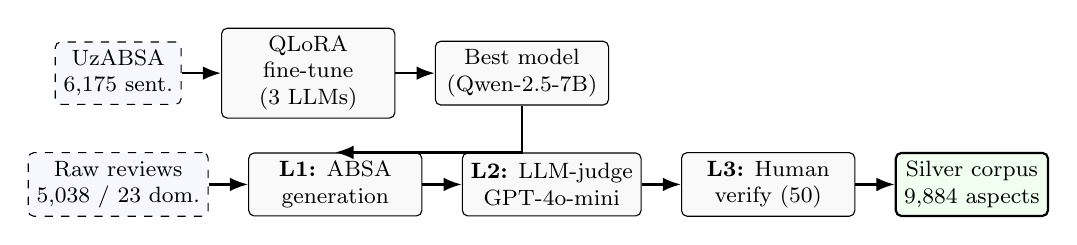
\begin{tikzpicture}[
  font=\footnotesize,
  node distance=6mm and 5mm,
  every node/.style={align=center},
  box/.style={draw, rounded corners=2pt, minimum height=8mm, minimum width=22mm, inner sep=3pt, fill=gray!5},
  data/.style={draw, dashed, rounded corners=2pt, minimum height=7mm, inner sep=3pt, fill=blue!3},
  outnode/.style={draw, thick, rounded corners=2pt, minimum height=8mm, inner sep=3pt, fill=green!6},
  arr/.style={-Latex, thick}
]
\node[data] (uzabsa) {UzABSA\\6{,}175 sent.};
\node[box, right=of uzabsa] (ft) {QLoRA\\fine-tune\\(3 LLMs)};
\node[box, right=of ft] (best) {Best model\\(Qwen-2.5-7B)};
\node[data, below=of uzabsa] (raw) {Raw reviews\\5{,}038 / 23 dom.};
\node[box, right=of raw] (l1) {\textbf{L1:} ABSA\\generation};
\node[box, right=of l1] (l2) {\textbf{L2:} LLM-judge\\GPT-4o-mini};
\node[box, right=of l2] (l3) {\textbf{L3:} Human\\verify (50)};
\node[outnode, right=of l3] (silver) {Silver corpus\\9{,}884 aspects};
\draw[arr] (uzabsa) -- (ft);
\draw[arr] (ft) -- (best);
\draw[arr] (best.south) |- (l1.north);
\draw[arr] (raw) -- (l1);
\draw[arr] (l1) -- (l2);
\draw[arr] (l2) -- (l3);
\draw[arr] (l3) -- (silver);
\end{tikzpicture}
\caption{End-to-end UzGenABSA pipeline. Three LLMs are QLoRA-fine-tuned
on UzABSA; the best (Qwen-2.5-7B) is re-deployed as an annotator for the
multi-domain raw corpus, gated by an LLM-as-Judge layer and calibrated by
a 50-review human verification step.}
\label{fig:pipeline}
\end{figure}

%====================================================================
\section{Experimental Setup}
\label{sec:setup}

\paragraph{Hardware and software.} All fine-tuning and inference runs use
a single NVIDIA RTX A6000 (48~GB VRAM, Ampere SM~8.6) under CUDA 12.8.
The stack is PyTorch 2.x, Transformers $\geq$ 4.45, TRL (SFTTrainer),
PEFT, bitsandbytes, Unsloth. Training experiments are logged to
Weights\,\&\,Biases; Figure~\ref{fig:wandb} shows the side-by-side W\&B
dashboard used during the campaign.

\begin{figure}[!htbp]
\centering
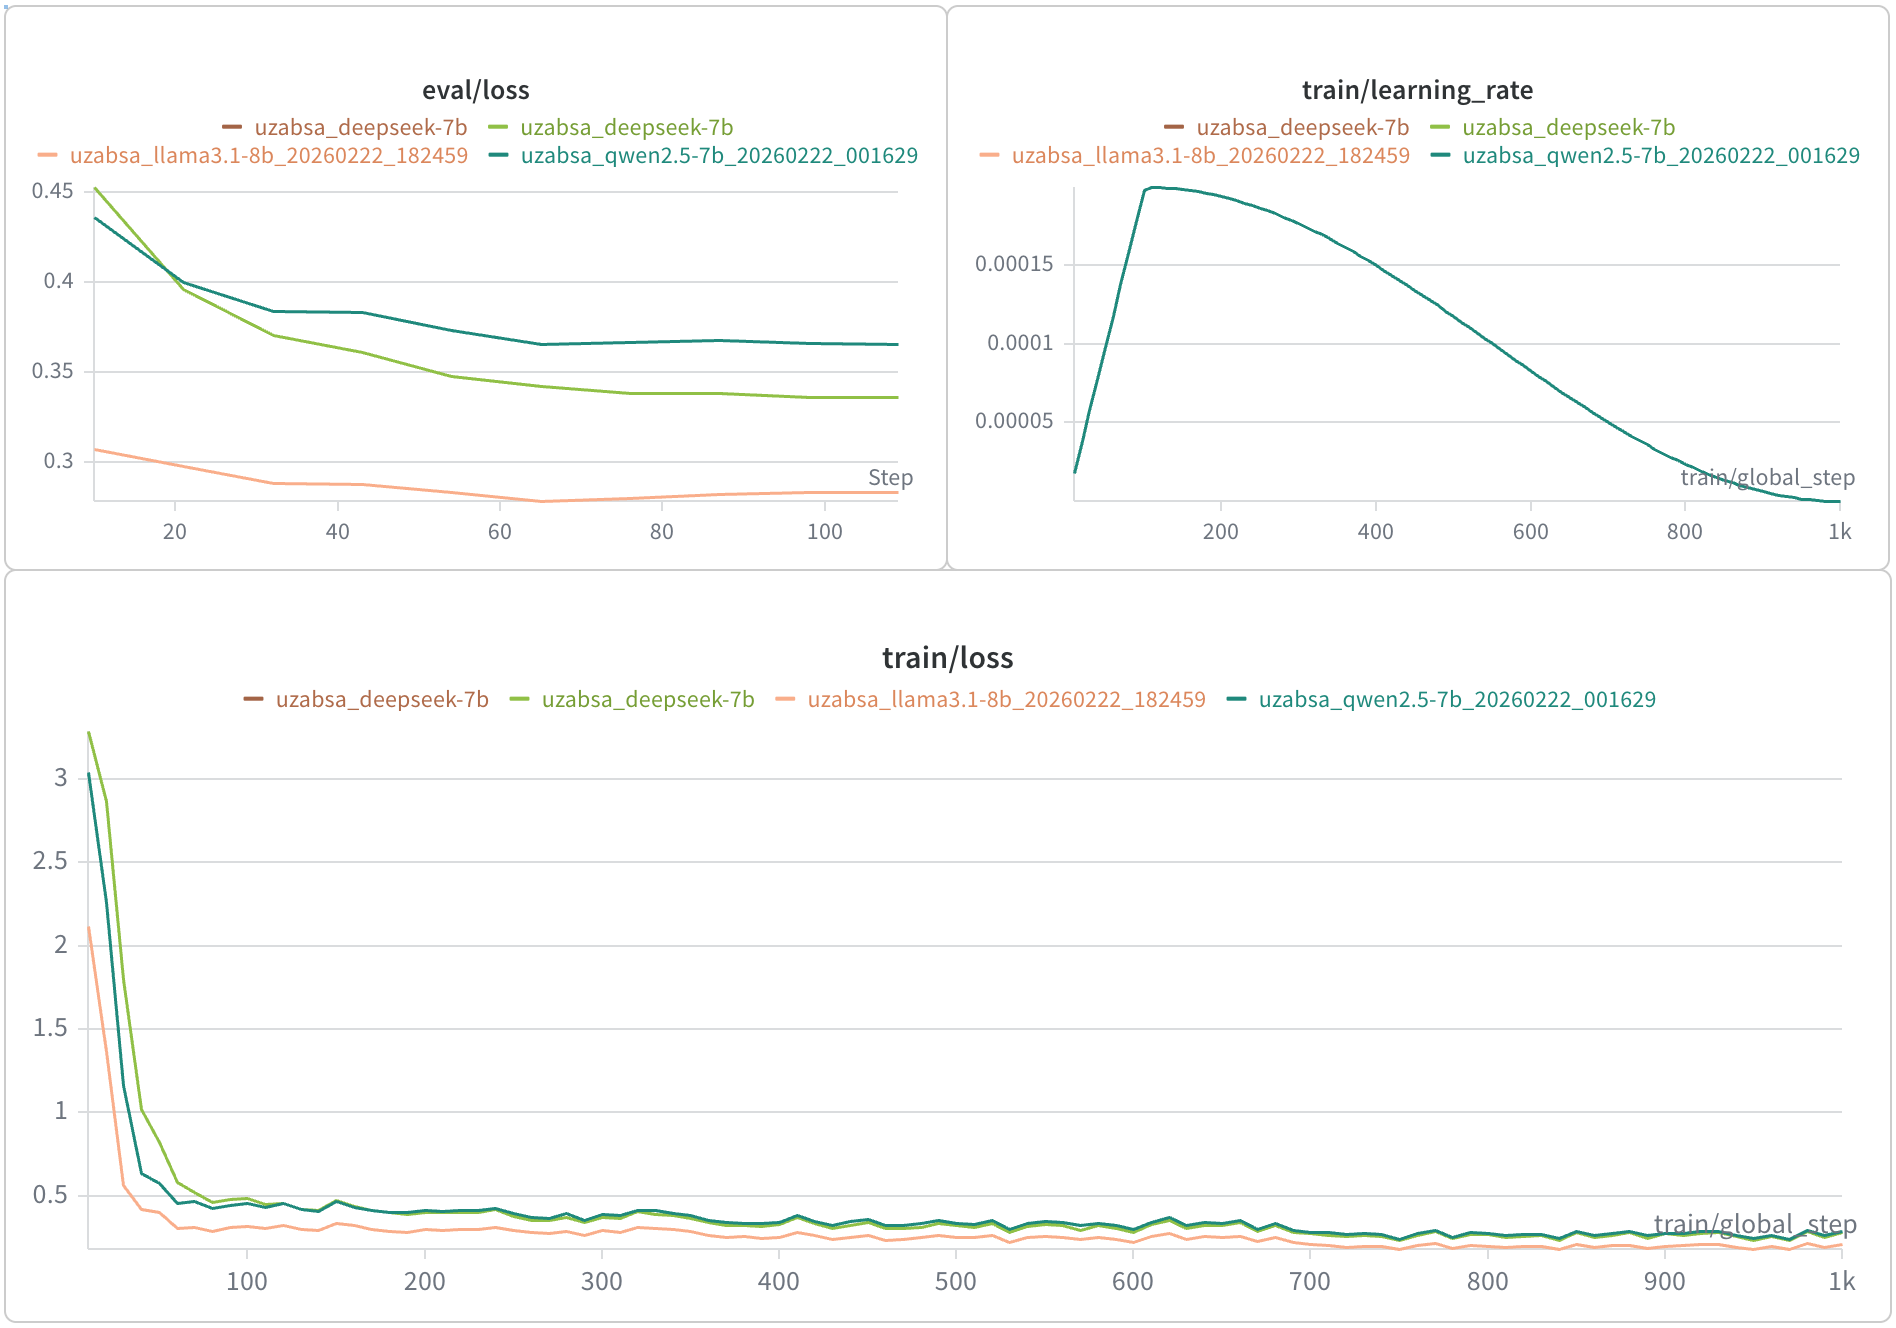
\includegraphics[width=0.95\textwidth]{wand-uzabsa.png}
\caption{Weights\,\&\,Biases dashboard for the three QLoRA fine-tuning
runs. Each model is trained for 1{,}000 steps under an identical
configuration; only the base model differs. The dashboard tracks training
loss, evaluation loss, learning-rate schedule, gradient norm and GPU
memory in real time, supporting the controlled comparison reported in
Section~\ref{sec:results:finetuned}.}
\label{fig:wandb}
\end{figure}

\paragraph{Metrics.} For ATE we report micro-averaged exact-match and
partial-match Precision/Recall/F1. For Aspect Sentiment Classification
(ASC) on matched aspect pairs we report accuracy and macro-F1. For
end-to-end ABSA we report the joint
\emph{aspect--polarity pair} F1 (E2E-F1), our primary metric. For TASD
(Target-Aspect-Sentiment Detection) we report micro-F1 over (term,
category, polarity) triples, restricted to the $\approx 75\%$ subset of
sentences where positional alignment between the term and category lists
is unambiguous. We always report the \emph{JSON parse success rate} as a
first-class metric: an unparseable output simply cannot enter downstream
analysis and must therefore be visible in the headline table. Greedy
decoding is used at evaluation time. Statistical comparisons are
bootstrapped over 1{,}000 resamples of the test set.

\paragraph{Baselines.} For each base model we run a zero-shot and a
3-shot baseline on the test split using the same Uzbek instruction prompt
as in fine-tuning; the 3-shot exemplars are sampled from train with
\texttt{seed=42} and kept fixed across all three models.

\paragraph{Judge configuration.} The judge is \texttt{gpt-4o-mini}
(temperature 0.0, deterministic decoding). Each judgement is a single
API call returning structured JSON. We re-prompt up to twice on parse
failure; remaining failures are excluded from aggregate statistics
(0 of 307 in our final run).

%====================================================================
\section{Results}
\label{sec:results}

\subsection{Tokenizer fertility on Uzbek}
\label{sec:results:fertility}

\begin{table}[!htbp]
\centering
\caption{Tokenizer fertility (tokens per whitespace-separated word) on
Uzbek text, computed on the UzABSA annotated set and on the 5{,}038-review
multi-domain corpus, broken down by dominant script. Lower is better.
Qwen-family tokenisers are markedly more compact on Uzbek-Latin than the
Llama tokeniser, especially in the Cyrillic buckets.}
\label{tab:fertility}
\renewcommand{\arraystretch}{1.1}
\setlength{\tabcolsep}{4pt}
\resizebox{\textwidth}{!}{%
\begin{tabular}{lcccc}
\toprule
\textbf{Tokenizer} & \textbf{Annotated} & \textbf{Uzbek-Latin} &
\textbf{Russian-Cyr.} & \textbf{Uzbek-Cyr.} \\
\midrule
Qwen-2.5-7B           & 1.71 & 1.74 & 1.95 & 2.18 \\
DeepSeek-R1-Distill-Qwen-7B & 1.72 & 1.75 & 1.96 & 2.19 \\
Llama-3.1-8B          & 2.03 & 2.07 & 2.42 & 2.71 \\
\bottomrule
\end{tabular}%
}
\end{table}

We measure tokenisation efficiency by the standard fertility metric --
tokens per whitespace-delimited word -- on both corpora and across the
three script buckets identified in Section~\ref{sec:data}. As
Table~\ref{tab:fertility} shows, the two Qwen-family tokenisers are
roughly $17\%$ more compact than Llama-3.1 on Uzbek-Latin and up to
$24\%$ more compact on Uzbek-Cyrillic. Fertility correlates with the
zero-shot baseline ATE-F1 (Section~\ref{sec:results:baselines}): Llama
under-performs Qwen at zero-shot despite a higher parameter count.
Importantly, however, the gap narrows substantially after fine-tuning
(Section~\ref{sec:results:finetuned}), showing that tokenizer disadvantage
is partially compensated by gradient-based adaptation -- a finding
consistent with cross-lingual transfer
results~\cite{blasi-etal-2022-systematic}.

\subsection{Zero-/few-shot baselines vs. fine-tuned}
\label{sec:results:baselines}

Table~\ref{tab:baselines} reports zero-shot and 3-shot results for the
three base models against their QLoRA-fine-tuned counterparts. Three
observations stand out. (i) \emph{Fine-tuning is the dominant factor}:
the smallest fine-tuning gain over 3-shot is $+0.30$ ATE-F1 (Llama). (ii)
\emph{Few-shot prompting helps modestly} ($+0.05$ to $+0.09$ ATE-F1 over
zero-shot), but does not close the gap with fine-tuning. (iii)
\emph{Instruction-following fails out of the box}: zero-shot JSON parse
rates are between 41\% and 72\%, vs. 95--100\% after fine-tuning. For
real-world annotation, this difference alone justifies the fine-tuning
cost.

\begin{table}[!htbp]
\centering
\caption{Zero-shot, 3-shot and fine-tuned ABSA performance on the
618-sentence held-out test split. ATE-F1 is exact-match; E2E-F1 is the
joint aspect--polarity pair F1; ``\%JSON'' is the JSON parse success
rate. Best per column in \textbf{bold}.}
\label{tab:baselines}
\renewcommand{\arraystretch}{1.1}
\setlength{\tabcolsep}{4pt}
\resizebox{\textwidth}{!}{%
\begin{tabular}{lccccccccc}
\toprule
& \multicolumn{3}{c}{\textbf{0-shot}} & \multicolumn{3}{c}{\textbf{3-shot}}
& \multicolumn{3}{c}{\textbf{Fine-tuned}} \\
\cmidrule(lr){2-4}\cmidrule(lr){5-7}\cmidrule(lr){8-10}
Model & ATE-F1 & E2E-F1 & \%JSON & ATE-F1 & E2E-F1 & \%JSON & ATE-F1 & E2E-F1 & \%JSON \\
\midrule
Qwen-2.5-7B          & 0.282 & 0.181 & 71.6 & 0.341 & 0.243 & 84.3 & \textbf{0.660} & 0.580 & \textbf{100.0} \\
Llama-3.1-8B         & 0.246 & 0.158 & 56.8 & 0.336 & 0.230 & 78.7 & 0.655 & \textbf{0.581} & 95.9 \\
DeepSeek-R1-Distill-7B & 0.207 & 0.122 & 41.4 & 0.291 & 0.187 & 67.2 & 0.603 & 0.502 & 95.4 \\
\bottomrule
\end{tabular}%
}
\end{table}

\subsection{Fine-tuned model comparison}
\label{sec:results:finetuned}

Table~\ref{tab:finetune} reports the controlled three-model comparison on
the full test set with matched training-efficiency figures. Qwen-2.5-7B is
the strongest aspect extractor (ATE-F1 0.660 exact, 0.770 partial) and
produces syntactically valid JSON on \emph{every} test sentence.
Llama-3.1-8B edges out Qwen on the joint aspect--polarity F1
(0.5805 vs.\ 0.5795) and on sentiment classification (accuracy 0.886,
macro-F1 0.844) but fails to produce parseable JSON on 4.1\% of inputs.
DeepSeek-R1-Distill underperforms its sibling Qwen-2.5 on every ABSA
metric despite \emph{better} validation cross-entropy than Qwen-2.5 --
a clear empirical illustration that loss-based model selection can
mislead for structured-output tasks. All three runs sit within an
8.5~GB GPU envelope (well under the A6000's 48~GB), so the choice is
driven by task metrics rather than compute.

\begin{table}[!htbp]
\centering
\caption{Fine-tuned three-model ABSA comparison on the 618-sentence
test split, with matched QLoRA training-efficiency figures. ``Pair F1''
is E2E aspect--polarity F1 (primary metric); ``Acc.''/``Mac-F1'' are
sentiment-classification metrics on matched pairs; ``Loss'' is the best
evaluation cross-entropy; ``Min'' is wall-clock training time.}
\label{tab:finetune}
\renewcommand{\arraystretch}{1.1}
\setlength{\tabcolsep}{4pt}
\resizebox{\textwidth}{!}{%
\begin{tabular}{lcccccccc}
\toprule
& \multicolumn{2}{c}{\textbf{ATE F1}} & & \multicolumn{2}{c}{\textbf{Sent.}} & & \multicolumn{2}{c}{\textbf{Train}} \\
\cmidrule(lr){2-3}\cmidrule(lr){5-6}\cmidrule(lr){8-9}
Model & Exact & Partial & \textbf{Pair F1} & Acc. & Mac-F1 & \%JSON & Loss & Min \\
\midrule
Qwen-2.5-7B            & \textbf{0.660} & \textbf{0.770} & 0.580 & 0.878 & 0.811 & \textbf{100.0} & 0.366 & \textbf{49.0} \\
Llama-3.1-8B           & 0.655 & 0.759 & \textbf{0.581} & \textbf{0.886} & \textbf{0.844} & 95.9 & \textbf{0.279} & 59.8 \\
DeepSeek-R1-Distill-7B & 0.603 & 0.728 & 0.502 & 0.832 & 0.772 & 95.4 & 0.336 & 62.3 \\
\bottomrule
\end{tabular}%
}
\end{table}

\paragraph{Loss-versus-task dissociation.} Llama owns the best validation
loss (0.279) but \emph{not} the best ATE-F1; DeepSeek owns better
validation loss than Qwen (0.336 vs.\ 0.366) but loses across all ABSA
metrics, in part because it over-predicts (predicted/reference ratio
1.29 vs.\ 1.16 for Qwen and 1.05 for Llama). The literature has documented
similar dissociations for QA and code
generation~\cite{10.1145/3777411}; we provide a clean Uzbek ABSA
counterpart and recommend reporting both loss \emph{and} downstream
metrics in low-resource fine-tuning studies.

\paragraph{TASD on the aligned subset.}
Because the UzABSA aspect-term and aspect-category lists are aligned in
$\approx 75\%$ of sentences (those with equal-length lists), we can
recover (term, category, polarity) triplets by positional alignment and
report TASD micro-F1. Llama is the strongest end-to-end predictor
(P/R/F1 $=$ 0.502/0.531/\textbf{0.516}), narrowly ahead of Qwen
(0.481/0.553/0.514) and well ahead of DeepSeek (0.398/0.510/0.447), in
line with the E2E Pair-F1 ranking above.

\subsection{Multi-domain LLM-as-Judge quality matrix}
\label{sec:results:judge}

We now move from the annotated test split to the open multi-domain
corpus. The best fine-tuned model (Qwen-2.5-7B, selected for ATE
recall and 100\% parse rate) is run over all 5{,}038 reviews,
producing 9{,}884 aspects with a polarity distribution of 75.1\%
positive / 16.5\% negative / 8.4\% neutral. A 307-review stratified
sample is then judged by GPT-4o-mini. Table~\ref{tab:judge-agg}
reports the aggregate scores and tier distribution;
Table~\ref{tab:judge-domain} reports per-domain Overall scores for the
sectors emphasised by this paper.

\begin{table}[!htbp]
\centering
\caption{LLM-as-Judge aggregate scores (1--5 scale; 307 stratified
reviews; GPT-4o-mini). Accuracy is high across the board; the
bottleneck is \emph{Completeness}, i.e.\ aspects that exist in the text
but are missed by the model.}
\label{tab:judge-agg}
\renewcommand{\arraystretch}{1.1}
\setlength{\tabcolsep}{8pt}
\begin{tabular}{lccccc|ccc}
\toprule
& \multicolumn{5}{c|}{\textbf{Mean dimension score (1--5)}} & \multicolumn{3}{c}{\textbf{Tier} (\%)} \\
& Comp. & Acc. & Sent. & Rel. & Overall & Incl. & Flag & Excl. \\
\midrule
Aggregate & 3.32 & \textbf{4.47} & 4.21 & 4.06 & 3.75 & 63.5 & 28.0 & 8.5 \\
\bottomrule
\end{tabular}
\end{table}

\begin{table}[!htbp]
\centering
\caption{Per-domain LLM-as-Judge Overall scores for the three sectors
foregrounded by this paper, plus selected near-domain and out-of-domain
comparisons. ``N'' is the per-domain sample size used by the judge.
Domains above the 3.5 inclusion threshold are shaded grey.}
\label{tab:judge-domain}
\renewcommand{\arraystretch}{1.1}
\setlength{\tabcolsep}{6pt}
\begin{tabular}{l|c|ccccc}
\toprule
\textbf{Domain} & \textbf{N} & Comp. & Acc. & Sent. & Rel. & \textbf{Overall} \\
\midrule
\multicolumn{7}{l}{\textit{HoReCa (in/near-domain for Layer 1)}} \\
Restoran/Ovqatlanish      & 50 & 3.68 & 4.76 & 4.56 & 4.66 & \textbf{4.24} \\
Oziq-ovqat do'konlari     & 15 & 3.47 & 4.33 & 4.47 & 4.13 & 3.80 \\
\midrule
\multicolumn{7}{l}{\textit{Retail}} \\
Elektron tijorat          & 21 & 3.43 & 4.48 & 4.10 & 4.14 & 3.81 \\
Gul/Sovg'a                & 12 & 3.08 & 4.08 & 4.83 & 3.67 & 3.58 \\
\midrule
\multicolumn{7}{l}{\textit{Banking and finance}} \\
Bank/Moliya               & 30 & 3.40 & 4.47 & 4.17 & 3.90 & 3.70 \\
To'lov tizimlari          & 24 & 3.00 & 4.29 & 4.38 & 3.54 & 3.54 \\
\midrule
\multicolumn{7}{l}{\textit{Other out-of-domain}} \\
Tibbiyot/Sog'liqni saqlash & 25 & 3.40 & 4.60 & 4.20 & 4.36 & 3.80 \\
Telekommunikatsiya         & 25 & 3.04 & 4.36 & 3.64 & 3.64 & 3.32 \\
Ta'lim                     & 20 & 2.90 & 4.20 & 3.80 & 3.45 & 3.25 \\
\bottomrule
\end{tabular}
\end{table}

Three patterns emerge. (a) The model trained on restaurant reviews
\emph{generalises} above the 3.5 inclusion threshold for 15 out of
23 domains, including the core retail (Elektron tijorat, Yetkazib
berish) and banking (Bank/Moliya, To'lov tizimlari) sectors. (b)
\emph{Accuracy} is uniformly high ($\geq 3.67/5$) across all domains:
when the model extracts an aspect, the aspect genuinely appears in the
text. The quality gradient is driven by \emph{Completeness} -- the
model misses domain-specific aspects rather than inventing wrong ones.
(c) The largest residual gap is in highly specialised verticals
(insurance, investment), where the lexical distance from restaurant
reviews is largest. We discuss the social-behavioural implications of
this gradient in Section~\ref{sec:discussion}.

\subsection{Human verification (Layer 3)}
\label{sec:results:human}

\begin{table}[!htbp]
\centering
\caption{Human verification on a 50-review subset, stratified across
domains and judge tiers. Authors independently labelled each review as
\textit{correct} (aspects accurately reflect text) or \textit{incorrect}.
Spearman $\rho$ is computed between the judge Overall score and the
binary human verdict on the same 50 reviews.}
\label{tab:human}
\renewcommand{\arraystretch}{1.1}
\setlength{\tabcolsep}{8pt}
\begin{tabular}{lc}
\toprule
\textbf{Quantity} & \textbf{Value} \\
\midrule
Reviews labelled                                    & 50 \\
Correct                                             & 47 / 50 (94.0\%) \\
Incorrect                                           & 3 / 50 (6.0\%) \\
Spearman $\rho$ (judge Overall vs.\ human verdict)  & 0.71 \\
\bottomrule
\end{tabular}
\end{table}

Table~\ref{tab:human} shows that 47 of 50 human-checked predictions are
substantively correct, and that the judge's Overall score correlates
strongly with the human verdict (Spearman $\rho = 0.71$). This supports
both the silver dataset's empirical quality and the use of the LLM judge
as a scalable proxy for human inspection, in line with prior
findings~\cite{10.5555/3666122.3668142}. The three failures are
concentrated in highly specialised verticals (one insurance, one
investment, one telecom), matching the per-domain gradient of
Section~\ref{sec:results:judge}.

%====================================================================
\section{Discussion: A Social-Behavioural Reading}
\label{sec:discussion}

\paragraph{What the silver corpus says about Uzbek service experience.}
Aggregated over 9{,}884 aspects, the silver corpus contains a striking
positivity bias (75.1\% positive). This mirrors the survivorship bias of
public review platforms (satisfied users post more reviews than
dissatisfied ones), but the 16.5\% negative class still encodes a clear
social signal once disaggregated by sector. In \textbf{HoReCa}, the most
frequent positive aspects are \textit{ovqat} (food quality) and
\textit{xizmat} (service), and the most frequent negatives are
\textit{narx} (price) and \textit{muhit} (ambience-related concerns
about cleanliness or noise). In \textbf{banking and fintech}, positives
concentrate on \textit{xizmat\_ko'rsatish} and \textit{ilova\_qulayligi}
(app usability), while negatives concentrate on \textit{tezlik}
(response speed) and \textit{kredit} (loan conditions). In \textbf{retail
and delivery}, positives concentrate on \textit{mahsulot\_sifati}
(product quality) and \textit{tezlik}, and negatives on
\textit{yetkazib\_berish} (delivery) and \textit{narx}. These patterns
are consistent with cross-cultural ABSA studies in other emerging
markets~\cite{electronics12030515} but provide the \emph{first}
Uzbek-language quantitative profile of which dimensions of service most
strongly drive (dis-)satisfaction.

\paragraph{Loss does not equal social signal, and completeness is the
bottleneck.} The Llama-vs-Qwen dissociation matters socially as well as
technically: a study selecting on lowest validation loss would have picked
Llama, missing the perfect-parse, higher-recall behaviour of Qwen that makes
the multi-domain annotation pipeline feasible at scale. The judge
dimensions (Table~\ref{tab:judge-agg}) further decompose the residual
error into a distinctive pattern: high accuracy and sentiment
correctness, lower completeness and relevance -- the model rarely
fabricates concerns citizens did not raise, but under-counts those they
did. Under-counting preserves precision at the cost of recall and
motivates domain-adaptive re-training as the most impactful future
direction.

\paragraph{Limitations.}
(i) UzABSA does not annotate opinion terms, so we cannot evaluate the
ASTE/ACOS/ASQP triplet/quad subtasks; this is shared with several
SemEval-2014-derived resources but is the largest single annotation gap.
(ii) Our silver dataset is annotated by a model fine-tuned on a single
domain; per-domain quality matters and is reported, but full gold
annotation for the non-HoReCa domains remains future work. (iii) The
LLM judge is itself fallible; we calibrate it against 50 human-verified
reviews but acknowledge the documented biases of LLM-judge
configurations~\cite{2506.22316}. (iv) The 5{,}058-review base corpus is
modest in absolute terms; expanding it is a priority for follow-up work
and is technically straightforward given the established pipeline.

%====================================================================
\section{Conclusion and Future Work}
\label{sec:conclusion}

We presented UzGenABSA, the first systematic study of LLM-based ABSA for
Uzbek. Under an identical QLoRA configuration, Qwen-2.5-7B, Llama-3.1-8B
and DeepSeek-R1-Distill-Qwen-7B were trained and benchmarked against their
own zero-/few-shot baselines. Fine-tuning dominates (zero-shot ATE-F1
$\approx 0.25$ vs.\ fine-tuned $\approx 0.66$), and Qwen vs.\ Llama trades
JSON robustness against sentiment accuracy. The strongest model was
re-deployed as an annotator over 5{,}038 multi-domain reviews, producing a
quality-tiered silver corpus of 9{,}884 aspects across 23 domains;
GPT-4o-mini judging plus a 50-review human-verification subset (47/50
correct, Spearman $\rho{=}0.71$) bound its empirical quality. We extract
the first Uzbek-language aspect-level satisfaction profile for banking,
retail and HoReCa and argue that validation cross-entropy is an unreliable
selection criterion for structured-output ABSA.

Future work targets three directions: (i) \emph{domain-adaptive ABSA}
incorporating the 119-subcategory taxonomy via self-training on the silver
dataset; (ii) \emph{opinion-term annotation} to enable ASTE/ACOS
evaluation; and (iii) \emph{cross-lingual transfer} to other Turkic
languages (Karakalpak, Kazakh, Kyrgyz, Turkmen) to test whether the
in-domain $\to$ specialised-domain gradient observed for Uzbek
replicates~\cite{blasi-etal-2022-systematic,uzbekendingssanat}.

\begin{credits}
\subsubsection{\ackname} We thank the \texttt{sharh.commeta.uz}
community whose public reviews made this study possible. Compute was
provided by the National University of Uzbekistan.

\subsubsection{\discintname} The authors have no competing interests to
declare that are relevant to the content of this article.
\end{credits}

%====================================================================
\FloatBarrier
\bibliographystyle{splncs04}
\bibliography{mybibliography}

\end{document}
